\documentclass{beamer}
\usetheme[white]{Wisconsin}
\usepackage{longtable}
\usepackage{listings}
\usepackage{color}
%% The amssymb package provides various useful mathematical symbols
\usepackage{amssymb}
%% The amsthm package provides extended theorem environments
\usepackage{amsthm} \usepackage{amsmath} \usepackage{tmadd,tmath}
\usepackage[mathcal]{euscript} \usepackage{color}
\usepackage{textcomp}
\usepackage{algorithm,algorithmic}
\definecolor{listinggray}{gray}{0.9}
\definecolor{lbcolor}{rgb}{0.9,0.9,0.9}
\lstset{
  backgroundcolor=\color{lbcolor},
  tabsize=4,
  rulecolor=,
  language=c++,
  basicstyle=\scriptsize,
  upquote=true,
  aboveskip={1.5\baselineskip},
  columns=fixed,
  showstringspaces=false,
  extendedchars=true,
  breaklines=true,
  prebreak =
  \raisebox{0ex}[0ex][0ex]{\ensuremath{\hookleftarrow}},
  frame=single,
  showtabs=false,
  showspaces=false,
  showstringspaces=false,
  identifierstyle=\ttfamily,
  keywordstyle=\color[rgb]{0,0,1},
  commentstyle=\color[rgb]{0.133,0.545,0.133},
  stringstyle=\color[rgb]{0.627,0.126,0.941},
}

%% colors
\setbeamercolor{boxheadcolor}{fg=white,bg=UWRed}
\setbeamercolor{boxbodycolor}{fg=black,bg=white}


%%---------------------------------------------------------------------------%%
\author{Stuart R. Slattery
  \\ Engineering Physics Department
  \\ University of Wisconsin - Madison
}

\date{\today} 
\title{A Spectral Analysis of the Domain Decomposed Monte Carlo Method
for Linear Systems}
\begin{document}
\maketitle

%%---------------------------------------------------------------------------%%
\begin{frame}{Monte Carlo Methods for Discrete Linear Systems}

  \begin{itemize}
  \item First proposed by J. Von Neumann and S.M. Ulam in the 1940's
    \medskip \medskip
  \item Earliest published reference in 1950
    \medskip \medskip
  \item General lack of published work
    \medskip \medskip
  \item Recent work by Evans and others has yielded new potential
    applications
    \medskip \medskip
  \item Domain decomposed parallelism has yet to be exploited - would
    like a preliminary analytic framework
  \end{itemize}

\end{frame}

%%---------------------------------------------------------------------------%%
\begin{frame}{Monte Carlo Linear Solver Preliminaries}

  \begin{itemize}
  \item Split the linear operator
  \end{itemize}

  \[
  \ve{H} = \ve{I} - \ve{A}
  \]

  \[
  \ve{A}\ve{x} = \ve{b} \ \ \ \rightarrow \ \ \ \ve{x} = \ve{H} \ve{x}
  + \ve{b}
  \]

  \medskip
  \begin{itemize}
  \item Generate the \textit{Neumann series}
  \end{itemize}
  
  \[
  \ve{A}^{-1} = (\ve{I}-\ve{H})^{-1} = \sum_{k=0}^{\infty} \ve{H}^k
  \]

  \medskip
  \begin{itemize}
  \item Require $\rho(\ve{H}) < 1$ for convergence
  \end{itemize}

  \[
  \ve{A}^{-1}\ve{b} = \sum_{k=0}^{\infty} \ve{H}^k\ve{b} = \ve{x}
  \]

\end{frame}

%%---------------------------------------------------------------------------%%
\begin{frame}{Monte Carlo Linear Solver Preliminaries}

  \begin{itemize}
  \item Expand the Neumann series
  \end{itemize}

  \[
  x_i = \sum_{k=0}^{\infty}\sum_{i_1}^{N}\sum_{i_2}^{N}\ldots
  \sum_{i_k}^{N}h_{i,i_1}h_{i_1,i_2}\ldots h_{i_{k-1},i_k}b_{i_k}
  \]

  \medskip
  \begin{itemize}
  \item Define a sequence of state transitions
  \end{itemize}
  
  \[
  \nu = i \rightarrow i_1 \rightarrow \cdots \rightarrow i_{k-1}
  \rightarrow i_{k}
  \]

  \medskip
  \begin{itemize}
  \item Define the \textit{Neumann-Ulam decomposition}\footnote{The
    Hadamard product $\ve{A} = \ve{B} \circ \ve{C}$ is defined
    element-wise as $a_{ij} = b_{ij} c_{ij}$.}
  \end{itemize}

  \[
  \ve{H} = \ve{P} \circ \ve{W}
  \]

\end{frame}

%%---------------------------------------------------------------------------%%
\begin{frame}{Adjoint Method}

  \begin{itemize}
  \item Solve the adjoint linear system
  \end{itemize}

  \[
  \ve{A}^T \ve{y} = \ve{d}
  \]

  \[
  \ve{y} = \ve{H}^T \ve{y} + \ve{d}
  \]

  \medskip
  \begin{itemize}
  \item Set the adjoint constraint
  \end{itemize}

  \[
  \langle \ve{A}^T \ve{x}, \ve{y} \rangle = \langle \ve{x}, \ve{A}
  \ve{y} \rangle
  \]

  \[
  \langle \ve{x}, \ve{d} \rangle = \langle \ve{y}, \ve{b} \rangle
  \]
  
\end{frame}

%%---------------------------------------------------------------------------%%
\begin{frame}{Adjoint Method}

  \begin{itemize}
  \item Generate the Neumann series for the adjoint operator
  \end{itemize}

  \[
  \ve{y} = (\ve{I} - \ve{H}^T)^{-1} \ve{d} = \sum_{k=0}^{\infty}
  (\ve{H}^T)^k\ve{d}
  \]

  \medskip
  \begin{itemize}
  \item Expand the series
  \end{itemize}

  \[
  y_i = \sum_{k=0}^{\infty}\sum_{i_1}^{N}\sum_{i_2}^{N}\ldots
  \sum_{i_k}^{N}h_{i_k,i_{k-1}}\ldots h_{i_2,i_1} h_{i_1,i} d_{i_k}
  \]

  \medskip
  \begin{itemize}
  \item Pick another constraint to yield the original solution
  \end{itemize}

  \[
  \ve{d} = \boldsymbol{\delta}_i,\ \langle \ve{y}, \ve{b} \rangle =
  \langle \ve{x}, \boldsymbol{\delta}_i \rangle = x_i
  \]
  
\end{frame}

%%---------------------------------------------------------------------------%%
\begin{frame}{Adjoint Method}

  \begin{itemize}
  \item Use the adjoint Neumann-Ulam decomposition
  \end{itemize}

  \[
  \ve{H}^{T} = \ve{P} \circ \ve{W}
  \]

  \[
  p_{ij} = \frac{|h_{ji}|}{\sum_j |h_{ji}|},\ w_{ij} =
  \frac{h_{ji}}{p_{ij}}
  \]

  \medskip
  \begin{itemize}
  \item Build the estimator and expectation value
  \end{itemize}

  \[
  X_j(\nu) = \sum_{m=0}^k W_{m} \delta_{i_m,j}
  \]

  \[
  \begin{split}
    E\{X_j\} &=\sum_{k=0}^{\infty}\sum_{i_1}^{N}\sum_{i_2}^{N}\ldots
    \sum_{i_k}^{N} b_{i_0} h_{i_0,i_1}h_{i_1,i_2}\ldots h_{i_{k-1},i_k}
    \delta_{i_k,j} \\ &= x_{j}
  \end{split}
  \]

\end{frame}

%%---------------------------------------------------------------------------%%
\begin{frame}{Adjoint Method: Evolution of a Solution}

  \begin{figure}[h!]
    \begin{center}
      \includegraphics[width=4in]{adjoint_1.png}
    \end{center}
    \caption{\textbf{Adjoint solution to Poisson Equation.}
      \textit{\sn{1}{0} total histories, 0.286 seconds CPU time.} }
  \end{figure}

\end{frame}

%%---------------------------------------------------------------------------%%
\begin{frame}{Adjoint Method: Evolution of a Solution}

  \begin{figure}[h!]
    \begin{center}
      \includegraphics[width=4in]{adjoint_10.png}
    \end{center}
    \caption{\textbf{Adjoint solution to Poisson Equation.}
      \textit{\sn{1}{1} total histories, 0.278 seconds CPU time.} }
  \end{figure}

\end{frame}

%%---------------------------------------------------------------------------%%
\begin{frame}{Adjoint Method: Evolution of a Solution}

  \begin{figure}[h!]
    \begin{center}
      \includegraphics[width=4in]{adjoint_100.png}
    \end{center}
    \caption{\textbf{Adjoint solution to Poisson Equation.}
      \textit{\sn{1}{2} total histories, 0.275 seconds CPU time.} }
  \end{figure}

\end{frame}

%%---------------------------------------------------------------------------%%
\begin{frame}{Adjoint Method: Evolution of a Solution}

  \begin{figure}[h!]
    \begin{center}
      \includegraphics[width=4in]{adjoint_1000.png}
    \end{center}
    \caption{\textbf{Adjoint solution to Poisson Equation.}
      \textit{\sn{1}{3} total histories, 0.291 seconds CPU time.} }
  \end{figure}

\end{frame}

%%---------------------------------------------------------------------------%%
\begin{frame}{Adjoint Method: Evolution of a Solution}

  \begin{figure}[h!]
    \begin{center}
      \includegraphics[width=4in]{adjoint_10000.png}
    \end{center}
    \caption{\textbf{Adjoint solution to Poisson Equation.}
      \textit{\sn{1}{4} total histories, 0.428 seconds CPU time.} }
  \end{figure}

\end{frame}

%%---------------------------------------------------------------------------%%
\begin{frame}{Adjoint Method: Evolution of a Solution}

  \begin{figure}[h!]
    \begin{center}
      \includegraphics[width=4in]{adjoint_100000.png}
    \end{center}
    \caption{\textbf{Adjoint solution to Poisson Equation.}
      \textit{\sn{1}{5} total histories, 1.76 seconds CPU time.} }
  \end{figure}

\end{frame}

%%---------------------------------------------------------------------------%%
\begin{frame}{Adjoint Method: Evolution of a Solution}

  \begin{figure}[h!]
    \begin{center}
      \includegraphics[width=4in]{adjoint_1000000.png}
    \end{center}
    \caption{\textbf{Adjoint solution to Poisson Equation.}
      \textit{\sn{1}{6} total histories, 15.1 seconds CPU time.} }
  \end{figure}

\end{frame}

%%---------------------------------------------------------------------------%%
\begin{frame}{Adjoint Method: Evolution of a Solution}

  \begin{figure}[h!]
    \begin{center}
      \includegraphics[width=4in]{adjoint_10000000.png}
    \end{center}
    \caption{\textbf{Adjoint solution to Poisson Equation.}
      \textit{\sn{1}{7} total histories, 149 seconds CPU time.} }
  \end{figure}

\end{frame}


%%---------------------------------------------------------------------------%%
\begin{frame}{Domain Decomposition}

  \begin{columns}
    \begin{column}{0.5\textwidth}
      \begin{itemize}
      \item Each parallel process owns a piece of the domain (linear
        system)
        \bigskip
      \item Random walks must be transported between adjacent domains
        through parallel communication
        \bigskip
      \item Domain decomposition determined by the input system
      \end{itemize}
    \end{column}

    \begin{column}{0.5\textwidth}
      \begin{figure}[htpb!]
        \begin{center}
          \scalebox{0.75}{ \input{msod_example.pdftex_t} }
        \end{center}
        \caption{\textbf{Domain decompostion example illustrating how
            domain-to-domain transport creates communication costs.}}
      \end{figure}
    \end{column}
  \end{columns}

\end{frame}

%%---------------------------------------------------------------------------%%
\begin{frame}{Model Problem - 2D Neutron Diffusion}

  \begin{columns}

    \begin{column}{0.5\textwidth}
      \begin{figure}[t!]
        \begin{center}
          \scalebox{0.5}{\input{stencil.pdftex_t}}
        \end{center}
        \caption{\textbf{Nine-point Laplacian stencil.}}
        \label{fig:stencil}
      \end{figure}
    \end{column}

    \begin{column}{0.5\textwidth}
      \begin{equation}
        -D \boldsymbol{\nabla}^2 \phi + \Sigma_a \phi = S
        \label{eq:diffusion_eq_simple}
      \end{equation}

      \begin{equation}
        \ve{D}\boldsymbol{\phi}=\ve{s}
        \label{eq:operator_system}
      \end{equation}
    \end{column}

  \end{columns}

  \begin{multline}
    -\frac{1}{6h^2}[4 \phi_{i-1,j} + 4 \phi_{i+1,j} + 4 \phi_{i,j-1} + 4
      \phi_{i,j+1} + \phi_{i-1,j-1}\\ + \phi_{i-1,j+1} + \phi_{i+1,j-1}
      + \phi_{i+1,j+1} - 20 \phi_{i,j}] + \Sigma_a \phi_{i,j} = s_{i,j}
    \label{eq:fd_system}
  \end{multline}

\end{frame}

%%---------------------------------------------------------------------------%%
\begin{frame}{Spectral Analysis}

\begin{equation}
  \Phi_{p,q}(x,y) = e^{2 \pi \imath p x} e^{2 \pi \imath q y}
  \label{eq:eigenfunction_form}
\end{equation}

\begin{multline}
  \ve{D}\Phi_{p,q}(x,y) = \lambda_{p,q}(\ve{D})
  =\\ -\frac{D}{6h^2}\Big[4 e^{-2 \pi \imath p h} + 4 e^{2 \pi \imath
      p h} + 4 e^{-2 \pi \imath q h} + 4 e^{2 \pi \imath q h} + e^{-2
      \pi \imath p h} e^{-2 \pi \imath q h} \\ + e^{-2 \pi \imath p h}
    e^{2 \pi \imath q h} + e^{2 \pi \imath p h} e^{-2 \pi \imath q h}
    + e^{2 \pi \imath p h} e^{2 \pi \imath q h} - 20\Big] + \Sigma_a
  \label{eq:deriv_diff_1}
\end{multline}

\begin{equation}
  \lambda_{p,q}(\ve{D}) = -\frac{D}{6h^2}[ 8 \cos(\pi p h) + 8
    \cos(\pi q h) + 4 \cos(\pi p h) \cos(\pi q h) - 20] + \Sigma_a
  \label{eq:deriv_diff_2}
\end{equation}

\end{frame}

%%---------------------------------------------------------------------------%%
\begin{frame}{Jacobi Preconditioned System}

\begin{equation}
  \ve{M}^{-1} \ve{D} \boldsymbol{\phi} = \ve{M}^{-1} \ve{s}
  \label{eq:precond_diffsion}
\end{equation}

\begin{equation}
  \alpha = \Bigg[\frac{10 D}{3 h^2} + \Sigma_a\Bigg]^{-1}
  \label{eq:jacobi_scaling}
\end{equation}

\begin{equation}
  \lambda_{p,q}(\ve{M}^{-1} \ve{D}) = \alpha \lambda_{p,q}(\ve{D})
  \label{eq:preconditioned_Eigenvalues}
\end{equation}

\begin{equation}
  \ve{H} = \ve{I} - \ve{M}^{-1} \ve{D}
  \label{eq:iteration_matrix}
\end{equation}

\begin{equation}
  \lambda_{p,q}(\ve{H}) = -\frac{\alpha D}{6h^2}[ 8 \cos(\pi p h) + 8
    \cos(\pi q h) + 4 \cos(\pi p h) \cos(\pi q h)]
  \label{eq:iteration_spectrum}
\end{equation}

\end{frame}

%%---------------------------------------------------------------------------%%
\begin{frame}{Iteration Matrix Spectrum Results}

\begin{equation}
  \rho(\ve{H}) = \frac{10 \alpha D}{3 h^2}
  \label{eq:iteration_radius}
\end{equation}

\begin{figure}[t!]
  \begin{center}
    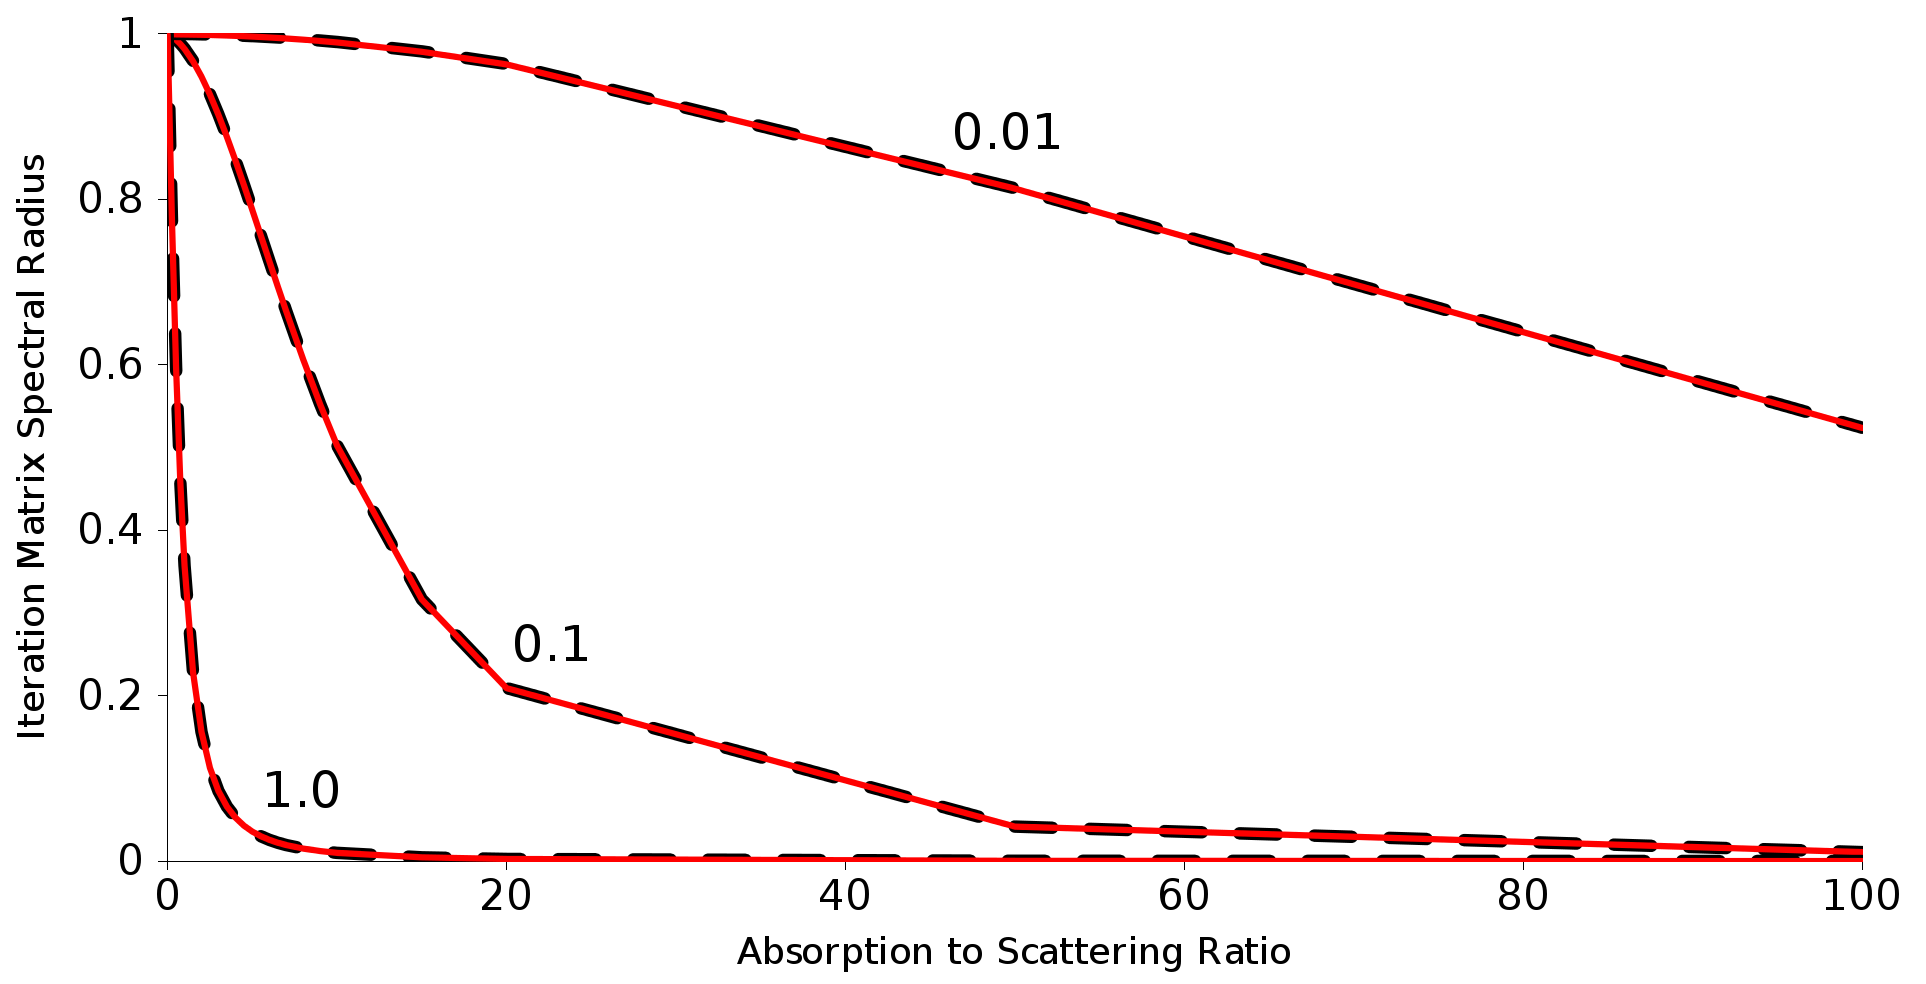
\includegraphics[width=3.5in,clip]{measured_spec_rad.png}
  \end{center}
  \caption{\textbf{Measured and analytic preconditioned diffusion
      operator spectral radius as a function of the absorption cross
      section to scattering cross section ratio.}}
  \label{fig:measured_spec_rad}
\end{figure}

\end{frame}

%%---------------------------------------------------------------------------%%
\begin{frame}{Random Walk Length}

\begin{equation}
  \ve{e}^{k} = \ve{H}^k\ve{e}^0
  \label{eq:linear_k_iter_error}
\end{equation}

\begin{equation}
  ||\ve{e}^{k}||_2 \leq \rho(\ve{H})^k \kappa(\ve{R})
  ||\ve{e}^0||_2
  \label{eq:linear_k_iter_norm2}
\end{equation}

\begin{equation}
  ||\ve{e}^{k}||_2 \leq \rho(\ve{H})^k ||\ve{e}^0||_2
  \label{eq:linear_k_iter_norm3}
\end{equation}

\begin{equation}
  ||\ve{e}^{k}||_2 = \epsilon ||\ve{e}^0||_2
  \label{eq:linear_k_iter_norm4}
\end{equation}

\begin{equation}
  k = \frac{ \log(W_c) }{ \log( \rho(\ve{H}) ) }
  \label{eq:analytic_k}
\end{equation}

\end{frame}

%%---------------------------------------------------------------------------%%
\begin{frame}{Random Walk Length Results}

\begin{figure}[t!]
  \begin{center}
    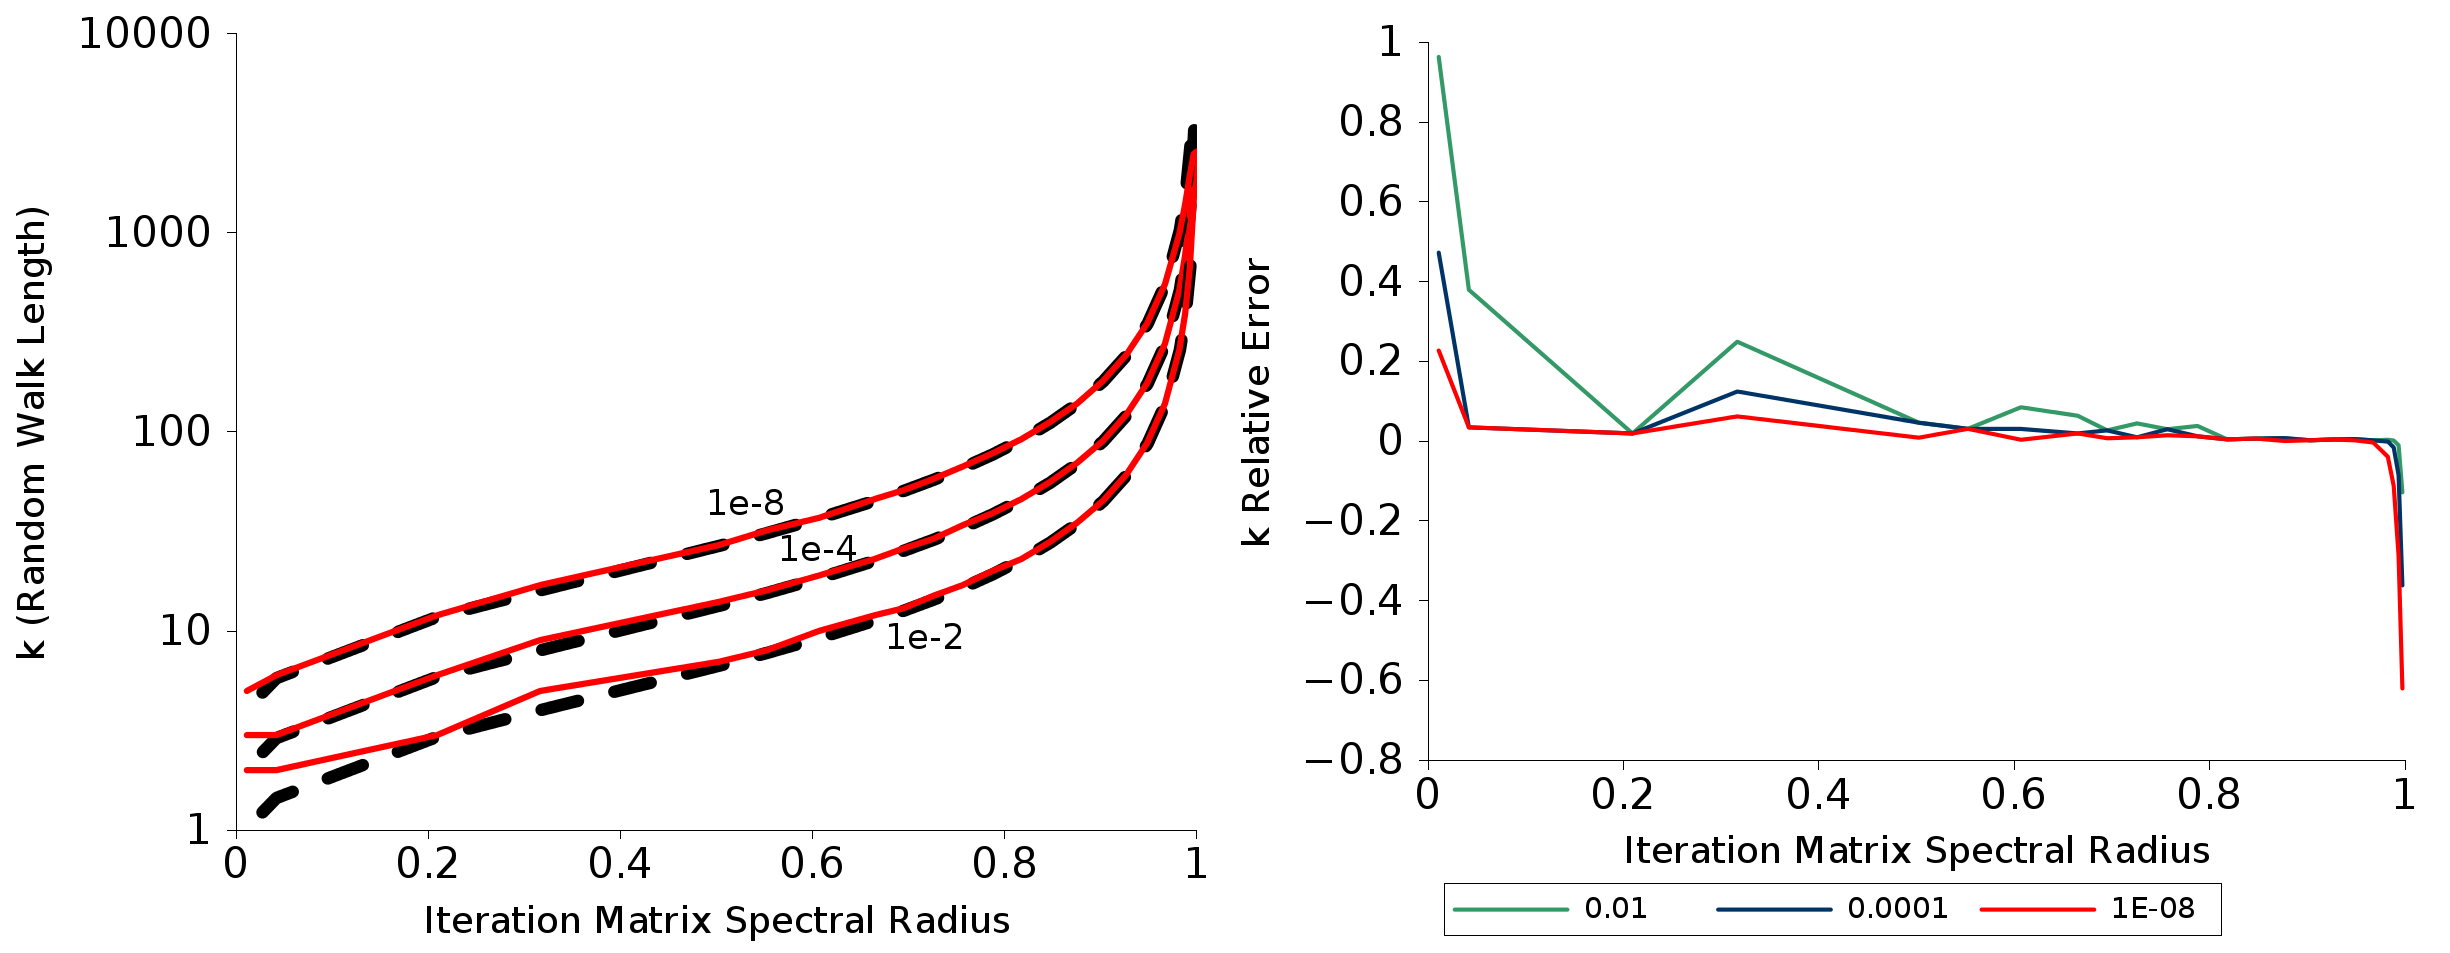
\includegraphics[width=4.5in,clip]{measured_length.png}
  \end{center}
  \caption{\textbf{Measured and analytic random walk length as a
      function of the iteration matrix spectral radius.}}
  \label{fig:measured_length}
\end{figure}

\end{frame}

%%---------------------------------------------------------------------------%%
\begin{frame}{Linear Operator Domain Optical Thickness}

  \begin{equation}
    \langle \bar{r_1^2} \rangle = (n_s h)^2 \ \ \ \rightarrow
    \ \ \ \langle \bar{r_k^2} \rangle = k (n_s h)^2
    \label{eq:step_1_length}
  \end{equation}

  \begin{equation}
    \langle \bar{r_k^2} \rangle = k \Bigg(\frac{n_s l}{n_i}\Bigg)^2
    \label{eq:step_k_length_sub}
  \end{equation}

  \begin{equation}
    \tau = \frac{l}{2 d \sqrt{\langle \bar{r_k^2} \rangle}}
      \label{eq:optical_thickness_1}
  \end{equation}

  \begin{equation}
    \tau = \frac{n_i}{2 d n_s \sqrt{k}}
    \label{eq:optical_thickness_2}
  \end{equation}

  \begin{equation}
    \tau = \frac{n_i}{2 d n_s}
    \sqrt{\frac{\log(\rho(\ve{H}))}{\log(W_c)}}
    \label{eq:optical_thickness_3}
  \end{equation}

\end{frame}

%%---------------------------------------------------------------------------%%
\begin{frame}{Domain Leakage Approximations}

  \begin{equation}
    \Lambda = \frac{average\ \#\ of\ particles\ leaving\ local\ domain}
            {total\ of\ \#\ of\ particles\ starting\ in\ local\ domain}
            \label{eq:leakage_fraction}
  \end{equation}

  \begin{equation}
    \Lambda = \frac{1}{1+\tau}
    \label{eq:wigner_domain_leakage}
  \end{equation}

  \begin{equation}
    \Lambda = \frac{1-e^{-\tau}}{\tau}
    \label{eq:mean_chord_domain_leakage}
  \end{equation}

\end{frame}

%%---------------------------------------------------------------------------%%
\begin{frame}{Domain Leakage Results}

  \begin{figure}[t!]
    \begin{center}
      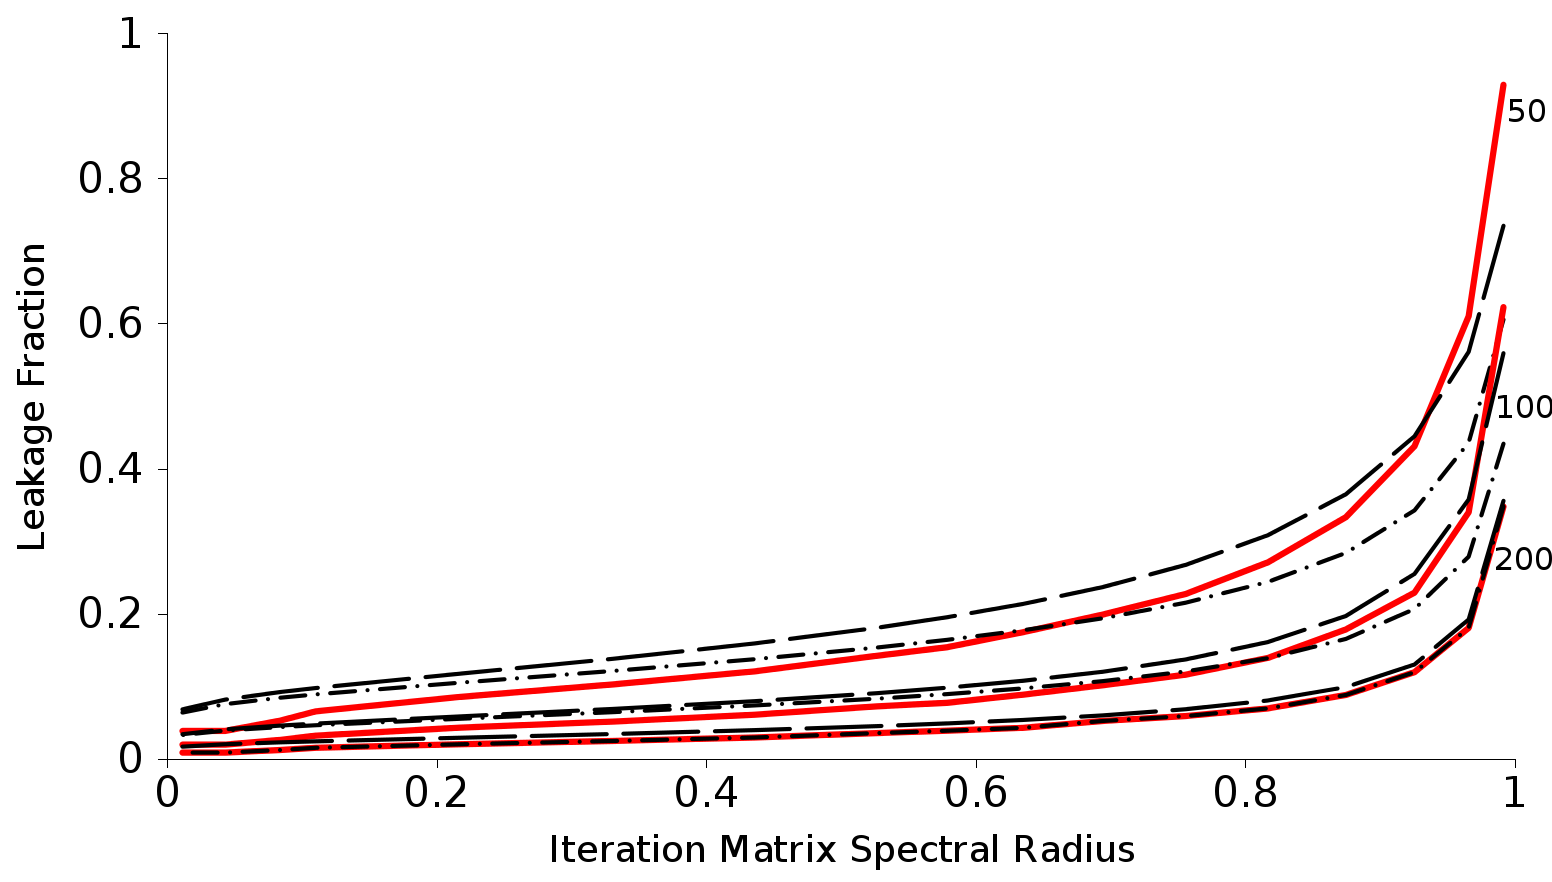
\includegraphics[width=3.5in,clip]{leakage_variation.png}
    \end{center}
    \caption{\textbf{Measured and analytic domain leakage as a function
        of the iteration matrix spectral radius.}}
    \label{fig:leakage_variation}
  \end{figure}

\end{frame}

%%---------------------------------------------------------------------------%%
\begin{frame}{Domain Leakage Results}

  \begin{figure}[ht!]
      \begin{center}
        \includegraphics[width=4.0in,clip]{leakage_error.png}
      \end{center}
      \caption{\textbf{Measured and analytic domain leakage absolute
          error as a function of the iteration matrix spectral radius.}}
      \label{fig:leakage_error}
  \end{figure}

\end{frame}

%%---------------------------------------------------------------------------%%
\begin{frame}{Conclusions}

\end{frame}

%%---------------------------------------------------------------------------%%

\end{document}
